% This code uses the tikz package
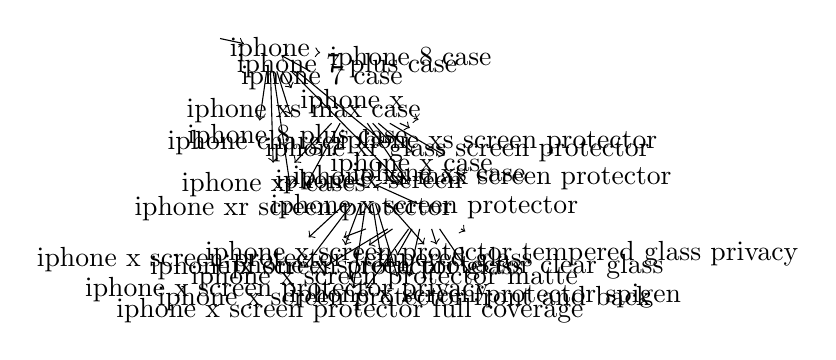
\begin{tikzpicture}
\node (v0) at (-0.0254,-0.272) {iphone x screen protector};
\node (v1) at (-0.732,0.0469) {iphone x screen};
\node (v2) at (-1.80,-0.940) {iphone x screen protector tempered glass};
\node (v3) at (-1.77,-1.32) {iphone x screen protector privacy};
\node (v4) at (-1.14,-1.04) {iphone x screen protector glass};
\node (v5) at (-0.974,-1.59) {iphone x screen protector full coverage};
\node (v6) at (-0.536,-1.17) {iphone x screen protector matte};
\node (v7) at (-0.284,-1.44) {iphone x screen protector front and back};
\node (v8) at (0.217,-1.03) {iphone x screen protector clear glass};
\node (v9) at (0.744,-1.40) {iphone x screen protector spigen};
\node (v10) at (0.956,-0.865) {iphone x screen protector tempered glass privacy};
\node (v11) at (-0.944,1.07) {iphone x};
\node (v12) at (-1.94,0.00705) {iphone xr cases};
\node (v13) at (-1.69,-0.290) {iphone xr screen protector};
\node (v14) at (-0.191,0.259) {iphone x case};
\node (v15) at (0.707,0.100) {iphone xs max screen protector};
\node (v16) at (0.154,0.140) {iphone xs case};
\node (v17) at (0.392,0.450) {iphone xr glass screen protector};
\node (v18) at (0.910,0.556) {iphone xs screen protector};
\node (v19) at (-1.99,1.73) {iphone};
\node (v20) at (-2.16,0.543) {iphone charger};
\node (v21) at (-1.64,0.622) {iphone 8 plus case};
\node (v22) at (-1.56,0.954) {iphone xs max case};
\node (v23) at (-1.33,1.37) {iphone 7 case};
\node (v24) at (-1.01,1.52) {iphone 7 plus case};
\node (v25) at (-0.201,1.61) {iphone 8 case};
\draw [->] (v0) edge (v2);
\draw [->] (v0) edge (v4);
\draw [->] (v0) edge (v3);
\draw [->] (v0) edge (v5);
\draw [->] (v0) edge (v6);
\draw [->] (v0) edge (v7);
\draw [->] (v0) edge (v8);
\draw [->] (v0) edge (v10);
\draw [->] (v0) edge (v9);
\draw [->] (v1) edge (v0);
\draw [->] (v1) edge (v2);
\draw [->] (v1) edge (v3);
\draw [->] (v1) edge (v4);
\draw [->] (v1) edge (v5);
\draw [->] (v1) edge (v6);
\draw [->] (v1) edge (v7);
\draw [->] (v1) edge (v8);
\draw [->] (v11) edge (v12);
\draw [->] (v11) edge (v15);
\draw [->] (v11) edge (v16);
\draw [->] (v11) edge (v13);
\draw [->] (v11) edge (v0);
\draw [->] (v11) edge (v14);
\draw [->] (v11) edge (v17);
\draw [->] (v11) edge (v18);
\draw [->] (v19) edge (v12);
\draw [->] (v19) edge (v20);
\draw [->] (v19) edge (v21);
\draw [->] (v19) edge (v13);
\draw [->] (v19) edge (v22);
\draw [->] (v19) edge (v0);
\draw [->] (v19) edge (v14);
\draw [->] (v19) edge (v23);
\draw [->] (v19) edge (v24);
\draw [->] (v19) edge (v25);
\end{tikzpicture}